%%%%%%%%%%%%%%%%%%%%%%%%%%%%%%%%%%%%%%%%%
% Journal Article
% LaTeX Template
% Version 1.4 (15/5/16)
%
% This template has been downloaded from:
% http://www.LaTeXTemplates.com
%
% Original author:
% Frits Wenneker (http://www.howtotex.com) with extensive modifications by
% Vel (vel@LaTeXTemplates.com)
%
% License:
% CC BY-NC-SA 3.0 (http://creativecommons.org/licenses/by-nc-sa/3.0/)
%
%%%%%%%%%%%%%%%%%%%%%%%%%%%%%%%%%%%%%%%%%

%----------------------------------------------------------------------------------------
%	PACKAGES AND OTHER DOCUMENT CONFIGURATIONS
%----------------------------------------------------------------------------------------

\documentclass[twoside,twocolumn]{article}

\usepackage{blindtext} % Package to generate dummy text throughout this template 

\usepackage[sc]{mathpazo} % Use the Palatino font
\usepackage[T1]{fontenc} % Use 8-bit encoding that has 256 glyphs
\linespread{1.05} % Line spacing - Palatino needs more space between lines
\usepackage{microtype} % Slightly tweak font spacing for aesthetics

\usepackage[english]{babel} % Language hyphenation and typographical rules

\usepackage[hmarginratio=1:1,top=32mm,columnsep=20pt]{geometry} % Document margins
\usepackage[hang, small,labelfont=bf,up,textfont=it,up]{caption} % Custom captions under/above floats in tables or figures
\usepackage{booktabs} % Horizontal rules in tables

\usepackage{lettrine} % The lettrine is the first enlarged letter at the beginning of the text

\usepackage{enumitem} % Customized lists
\setlist[itemize]{noitemsep} % Make itemize lists more compact

\usepackage{abstract} % Allows abstract customization
\renewcommand{\abstractnamefont}{\normalfont\bfseries} % Set the "Abstract" text to bold
\renewcommand{\abstracttextfont}{\normalfont\small\itshape} % Set the abstract itself to small italic text

\usepackage{titlesec} % Allows customization of titles
\renewcommand\thesection{\Roman{section}} % Roman numerals for the sections
\renewcommand\thesubsection{\roman{subsection}} % roman numerals for subsections
\titleformat{\section}[block]{\large\scshape\centering}{\thesection.}{1em}{} % Change the look of the section titles
\titleformat{\subsection}[block]{\large}{\thesubsection.}{1em}{} % Change the look of the section titles

\usepackage{fancyhdr} % Headers and footers
\pagestyle{fancy} % All pages have headers and footers
\fancyhead{} % Blank out the default header
\fancyfoot{} % Blank out the default footer
\fancyhead[C]{Harvey Hughes $\bullet$ November 2018 $\bullet$ Emmanuel College} % Custom header text
\fancyfoot[RO,LE]{\thepage} % Custom footer text

\usepackage{titling} % Customizing the title section

\usepackage{hyperref} % For hyperlinks in the PDF

\usepackage{graphicx}
\graphicspath{ {images/} }

\newenvironment{reusefigure}[2][htbp]
  {\addtocounter{figure}{-1}%
   \renewcommand{\theHfigure}{dupe-fig}% If you're using hyperref
   \renewcommand{\thefigure}{\ref{#2}}% Figure counter is \ref
   \renewcommand{\addcontentsline}[3]{}% Avoid placing figure in LoF
   \begin{figure}[#1]}
  {\end{figure}}
\usepackage{wrapfig}

%----------------------------------------------------------------------------------------
%	TITLE SECTION
%----------------------------------------------------------------------------------------

\setlength{\droptitle}{-4\baselineskip} % Move the title up

\pretitle{\begin{center}\Huge\bfseries} % Article title formatting
\posttitle{\end{center}} % Article title closing formatting
\title{Flight Control 3F1 } % Article title
\author{%
\\
\textsc{Harvey Hughes} \\
\normalsize Emmanuel College \\ % Your institution
\normalsize Lab Date : 14/11/18 \\
\normalsize \href{mailto:hh458@cam.ac.uk}{hh458@cam.ac.uk} % Your email address
}
\date{\today} % Leave empty to omit a date
\renewcommand{\maketitlehookd}{%
\begin{abstract}
\noindent
\blindtext
\newline
\end{abstract}
}

%----------------------------------------------------------------------------------------

\begin{document}

% Print the title
\maketitle

%----------------------------------------------------------------------------------------
%	ARTICLE CONTENTS
%----------------------------------------------------------------------------------------

\section{Introduction}

\lettrine[nindent=0em,lines=3]{O}   
safafdasf
%------------------------------------------------


\section{Results and Discussion}
\subsection{2.0 Manual control}
\begin{figure}[h]
  \centering
    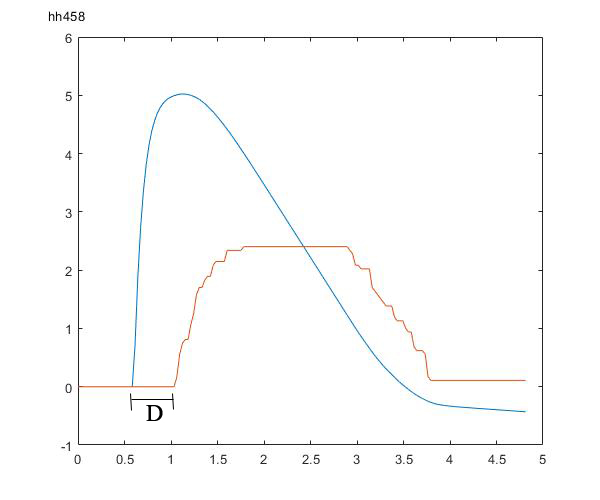
\includegraphics[width=\linewidth]{2_impulse}
  \caption{Typical response of manual control with a impulse disturbance of 5 }
  \label{fig:2impulse}
\end{figure}

\begin{figure}[h]
  \centering
    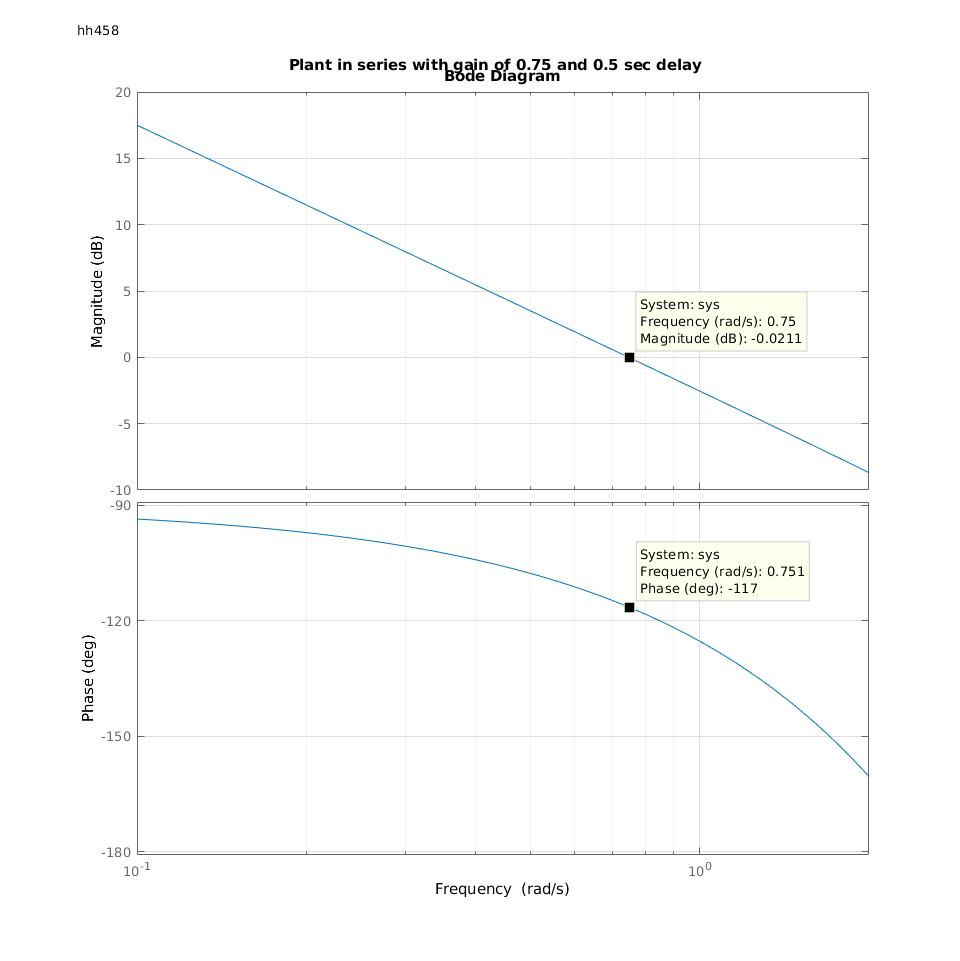
\includegraphics[width=\linewidth]{2_zoomed_in_bode}
  \caption{Bode plot of the controller with time delay 0.5 and gain 0.75 }
  \label{fig:2bode}
\end{figure}

\begin{figure}[h]
  \centering
    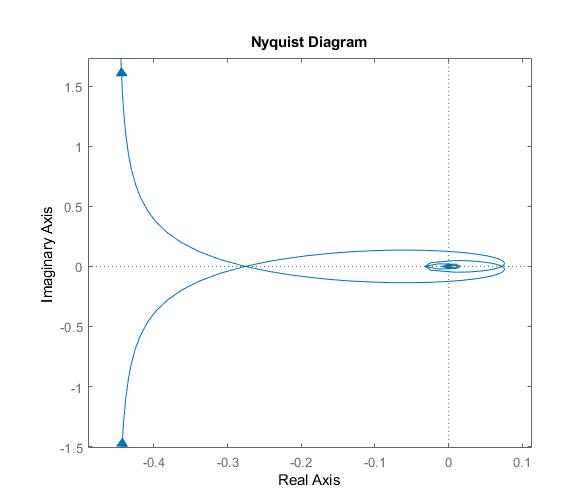
\includegraphics[width=\linewidth]{2_nyquist}
  \caption{Nyquist diagram sketch based off the response in figure \ref{fig:2bode} }
  \label{fig:2nyquist}
\end{figure}

\begin{figure}[h]
  \centering
    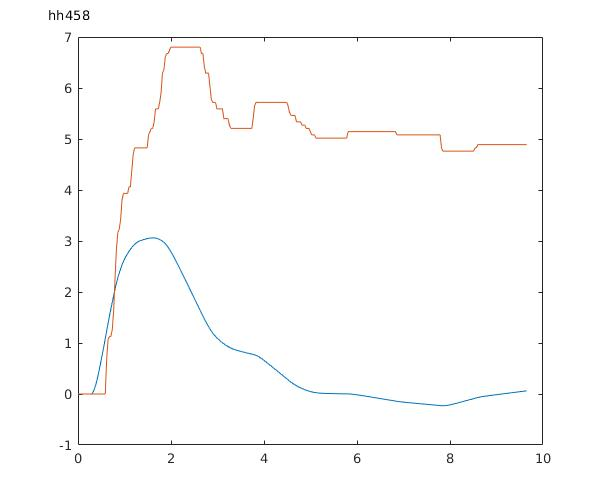
\includegraphics[width=\linewidth]{2_step}
  \caption{Typical response of manual control with a step disturbance of 5 }
  \label{fig:2step}
\end{figure}
%-------------------------------------
\subsection{2.1 Pilot induced oscillation}
 \begin{figure}[h]
  \centering
    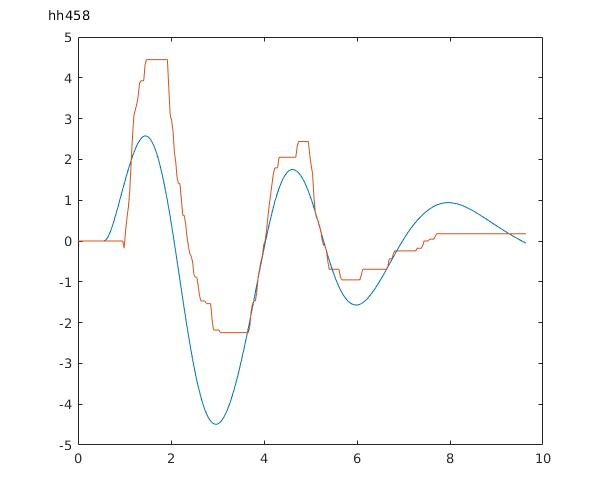
\includegraphics[width=\linewidth]{2-1_with_input}
  \caption{Typical response of pilot induced oscillations caused by attempting to stabilise the plane}
  \label{fig:2-1pio}
\end{figure}

 \begin{figure}[h]
  \centering
    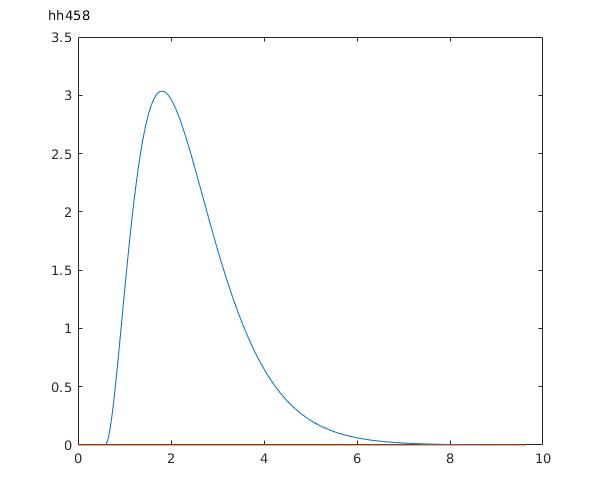
\includegraphics[width=\linewidth]{2-1_zero_input}
  \caption{Typical response of when no input is provided by the pilot, showing no oscillations}
  \label{fig:2-1zero}
\end{figure}

\begin{figure}[h]
  \centering
    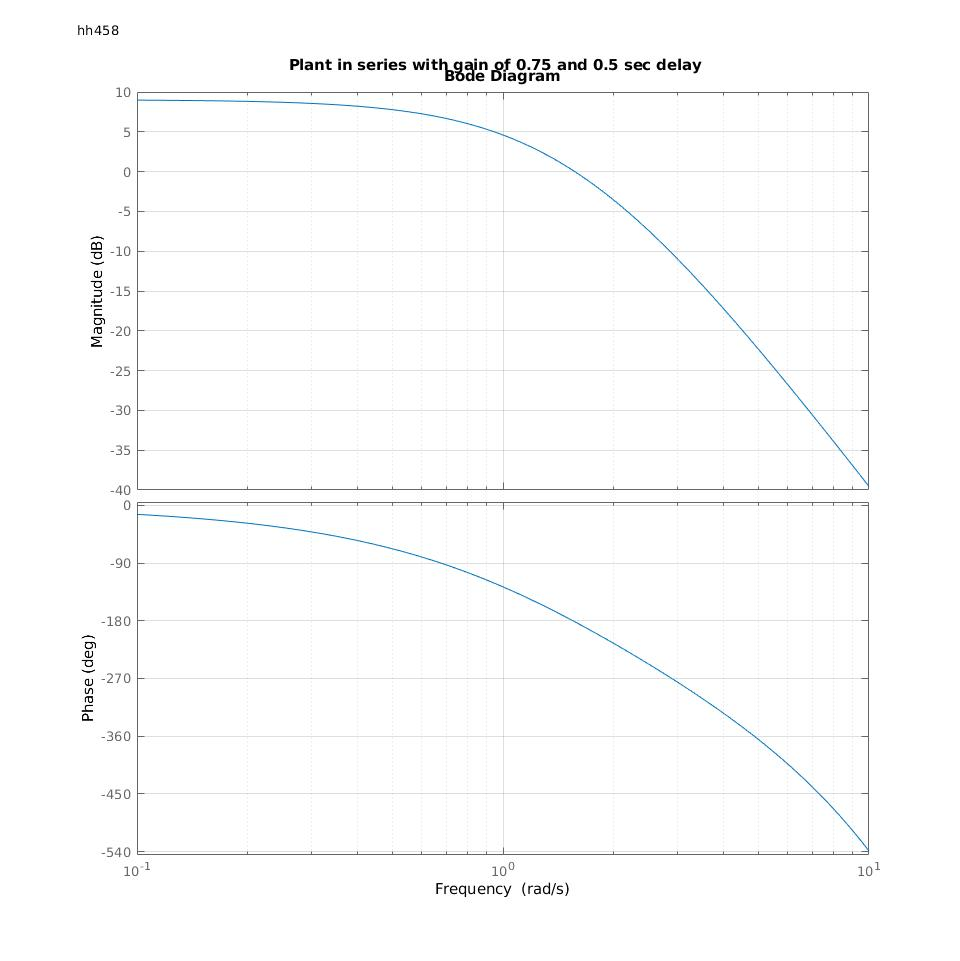
\includegraphics[width=\linewidth]{2-1_bode}
  \caption{Bode plot of the open loop response of the controller that caused PIO}
  \label{fig:2-1bode}
\end{figure}
%-------------------------------------
\subsection{2.2 Sinusoidal disturbances}
\begin{figure}[h]
  \centering
    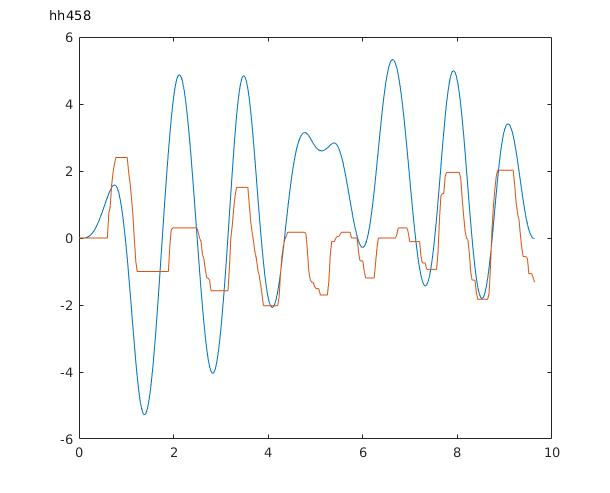
\includegraphics[width=\linewidth]{2-2}
  \caption{Typical response of attempting to stabilise a sinusoidal disturbance}
  \label{fig:2-2input}
\end{figure}

\begin{figure}[h]
  \centering
    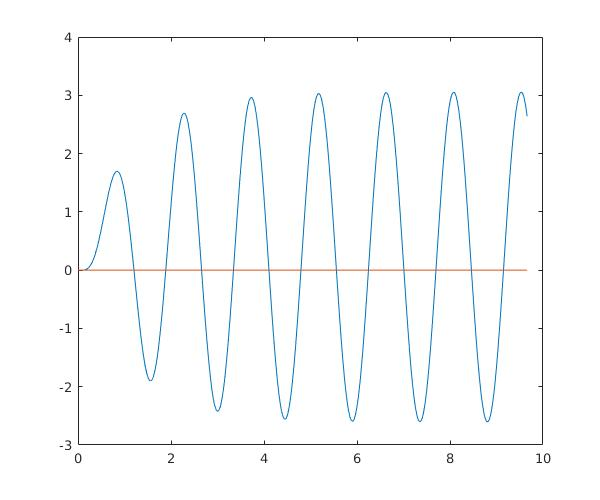
\includegraphics[width=\linewidth]{2-2-2}
  \caption{Typical response of a sinusoidal disturbance with no pilot input}
  \label{fig:2-2zero}
\end{figure}

\begin{figure}[h]
  \centering
    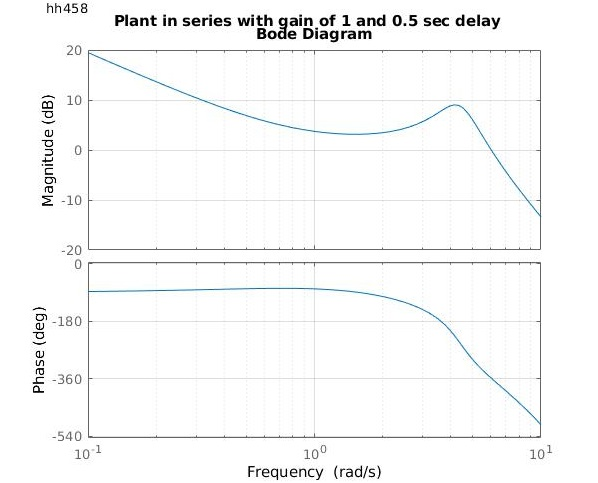
\includegraphics[width=\linewidth]{2-2_bode}
  \caption{Bode plot of the aircraft used for sinusoidal disturbances with gain 1 and delay 0.5}
  \label{fig:2-2bode}
\end{figure}
%-------------------------------------
\subsection{2.3 Unstable aircraft}
\begin{figure}[h]
  \centering
    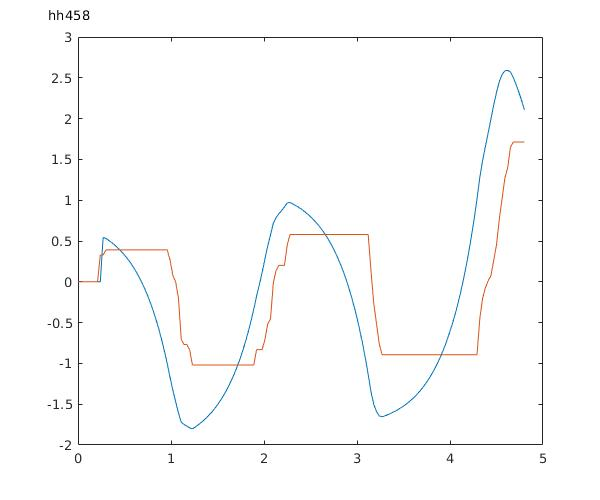
\includegraphics[width=\linewidth]{2-3_T=0-35}
  \caption{Response of stabilising the fastest pole in an unstable aircraft, with pole at T=0.35}
  \label{fig:2-3fastest}
\end{figure}

\begin{figure}[h]
  \centering
    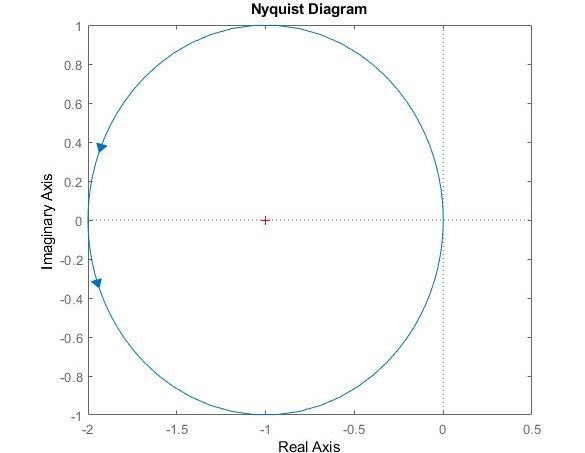
\includegraphics[width=\linewidth]{2-3_nyquist}
  \caption{Nyquist diagram for the unstable aircraft}
  \label{fig:2-3nyquist}
\end{figure}
%-------------------------------------
\subsection{3.0 Autopilot}
\begin{figure}[h]
  \centering
    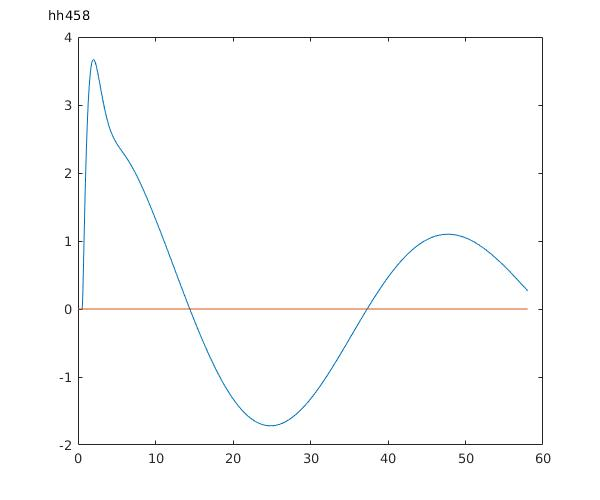
\includegraphics[width=\linewidth]{3_min_wait}
  \caption{Lightly damped phugoid motion under no input observed before an autopilot is constructed }
  \label{fig:3phugoid}
\end{figure}

\begin{figure}[h]
  \centering
    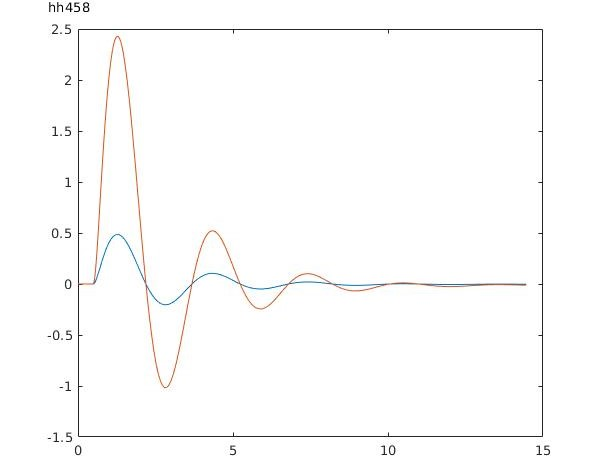
\includegraphics[width=\linewidth]{3_kp=5}
  \caption{Typical response when a proportional controller with gain 5 is implemented}
  \label{fig:3kp5}
\end{figure}

\begin{figure}[h]
  \centering
    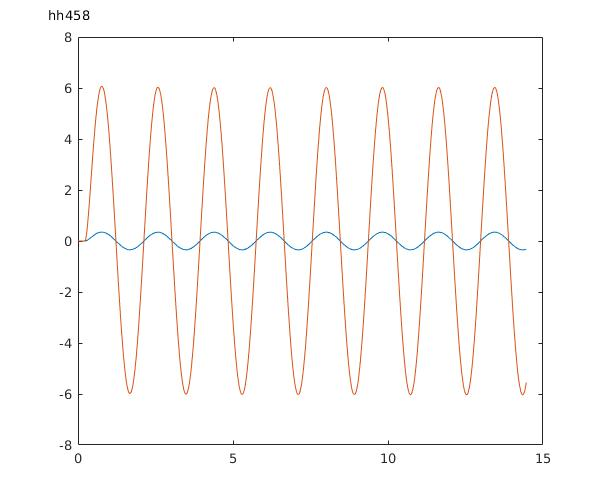
\includegraphics[width=\linewidth]{3_kp=17-4}
  \caption{Typical response when a proportional controller with gain 17.4 is implemented}
  \label{fig:3kp17-4}
\end{figure}
%-------------------------------------
\subsection{3.1 PID controller}
\begin{figure}[h]
  \centering
    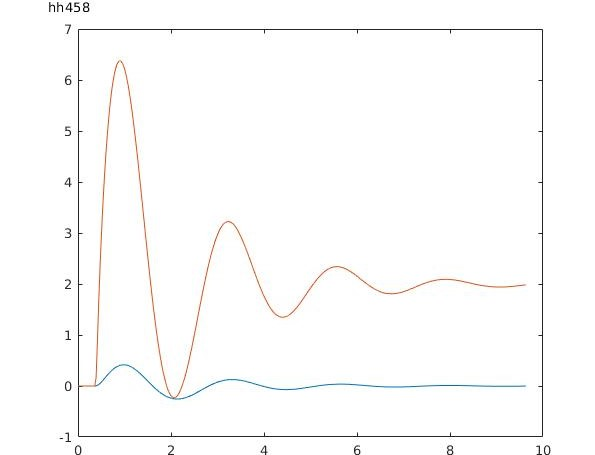
\includegraphics[width=\linewidth]{3-1_first_kd}
  \caption{Typical response when a PID controller is implemented with $K_p = 10.44,\:T_i=0.9,\:T_d=0.225$, the disturbance is an impulse and step of magnitude 2}
  \label{fig:3-1first}
\end{figure}

\begin{figure}[h]
  \centering
    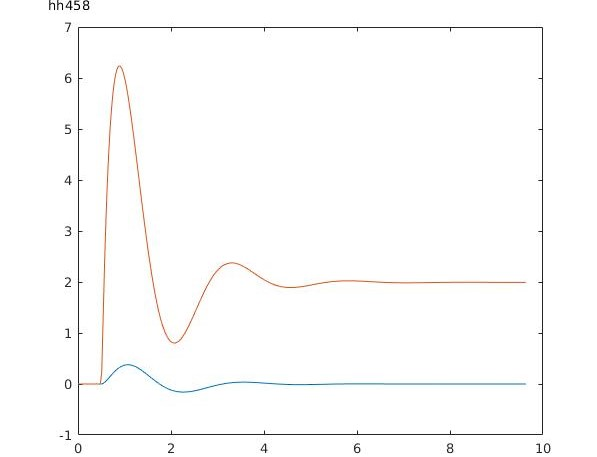
\includegraphics[width=\linewidth]{3-1_increased_kd}
  \caption{Typical response when a PID controller is implemented with $K_p = 10.44,\:T_i=0.9,\:T_d=0.315$ which is a 40\% increase to derivative gain, the disturbance is an impulse and step of magnitude 2}
  \label{fig:3-1increased}
\end{figure}
%-------------------------------------
\subsection{3.2 Integrator wind-up}
\begin{figure}[h]
  \centering
    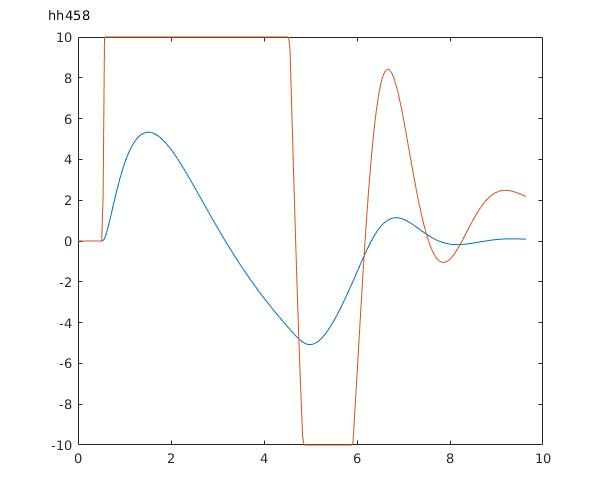
\includegraphics[width=\linewidth]{3-2_first_go}
  \caption{Typical response when a PID controller is implemented with $K_p = 10.44,\:T_i=0.9,\:T_d=0.315$, to a step disturbance of magnitude 2 and impulse magnitude 20}
  \label{fig:3-2first}
\end{figure}

\begin{figure}[h]
  \centering
    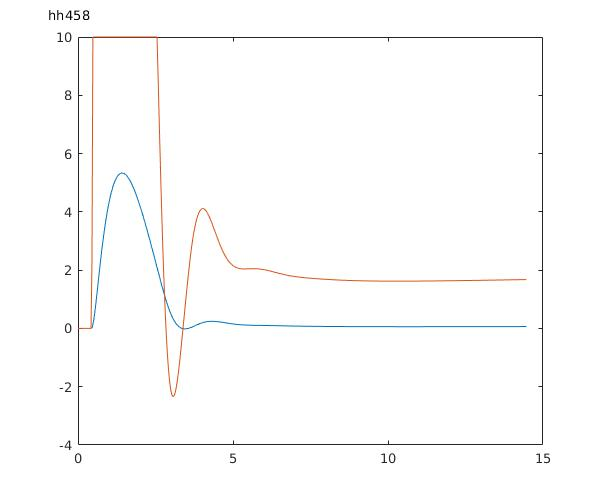
\includegraphics[width=\linewidth]{3-2_0-086}
  \caption{Typical response when a PID controller is implemented with $K_p = 10.44,\:T_i=0.9,\:T_d=0.315$, to a step disturbance of magnitude 2 and impulse magnitude 20 with integrator wind up capped at 0.086}
  \label{fig:3-20-086}
\end{figure}
%-------------------------------------
%------------------------------------------------

\section{Conclusion}


%------------------------------------------------
\section{Appendix}


%------------------------------------------------
\end{document}
